\documentclass[10pt, conference, letterpaper]{IEEEtran}
\IEEEoverridecommandlockouts

% Times New Roman Font Configuration (IEEE Standard)
\usepackage{newtxtext,newtxmath}

% Essential IEEE Packages
\usepackage{cite}
\usepackage{amsmath,amssymb,amsfonts}
\usepackage{graphicx}
\usepackage{textcomp}
\usepackage{xcolor}
\usepackage{booktabs}
\usepackage{tabularx}
\usepackage{url}
\usepackage[colorlinks=true, linkcolor=black, citecolor=black, urlcolor=blue]{hyperref}
\usepackage{microtype}
\usepackage{enumitem}
\usepackage{tikz}
\usetikzlibrary{shapes.geometric, arrows.meta, positioning, fit, backgrounds, calc}

% Custom column types for clean table alignment
\newcolumntype{Y}{>{\raggedright\arraybackslash}X}
\newcolumntype{C}{>{\centering\arraybackslash}X}

% Standard IEEE float spacing & padding for clean 6-page fit
\setlength{\textfloatsep}{5pt plus 1pt minus 1pt}
\setlength{\floatsep}{4pt plus 1pt minus 1pt}
\setlength{\intextsep}{4pt plus 1pt minus 1pt}
\setlength{\abovecaptionskip}{3pt}
\setlength{\belowcaptionskip}{2pt}

% BibTeX fix
\def\BibTeX{{\rm B\kern-.05em{\sc i\kern-.025em b}\kern-.08em
    T\kern-.1667em\lower.7ex\hbox{E}\kern-.125emX}}

\begin{document}

% Paper Title
\title{\LARGE\bfseries AI-Driven Personalized Nutrition Assistant with Adaptive Meal Planning and Health Monitoring}

% Author Block (IEEE Conference Format with balanced email sizing)
\author{
\IEEEauthorblockN{Sriram Ganesh M}
\IEEEauthorblockA{\textit{Department of Information Technology} \\
\textit{Rajalakshmi Engineering College} \\
Chennai, India \\
\href{mailto:231001213@rajalakshmi.edu.in}{\footnotesize\textcolor{blue}{\underline{231001213@rajalakshmi.edu.in}}}}
\and
\IEEEauthorblockN{Vishal T}
\IEEEauthorblockA{\textit{Department of Information Technology} \\
\textit{Rajalakshmi Engineering College} \\
Chennai, India \\
\href{mailto:231001249@rajalakshmi.edu.in}{\footnotesize\textcolor{blue}{\underline{231001249@rajalakshmi.edu.in}}}}
\and
\IEEEauthorblockN{Mrs. A.P. Aruna Jameela}
\IEEEauthorblockA{\textit{Department of Information Technology} \\
\textit{Rajalakshmi Engineering College} \\
Chennai, India \\
\href{mailto:arunajameela.ap@rajalakshmi.edu.in}{\footnotesize\textcolor{blue}{\underline{arunajameela.ap@rajalakshmi.edu.in}}}}
}

\maketitle

% Abstract
\begin{abstract}
Eating healthy is one of the best ways to feel energetic and manage chronic conditions like diabetes and high blood pressure. Yet most existing nutrition apps only count calories after meals are already eaten, give generic advice that ignores daily physical work, and fail to suggest practical meals that fill specific nutrient shortages. In this paper, we present \textbf{MealMentor (NutriSense AI)}, an easy-to-use, AI-powered nutrition assistant designed to give clear, personalized, and safe dietary guidance. Rather than using confusing black-box models, MealMentor starts with reliable health rules: it calculates resting calorie burn using the Mifflin--St Jeor formula, adjusts targets to real jobs using an Indian occupation matcher, and sets safe medical limits for diabetes (capping free sugars at 25~g) and hypertension (limiting sodium to 1500~mg). The system tracks active daily shortages across ten nutrients (protein, carbs, fat, fiber, calcium, iron, vitamin C, sugar, and sodium). To make logging food effortless, users can snap a photo of their plate using Google Gemini Vision, scan a packaged food barcode with an offline 500-item cache, or speak naturally using browser-native voice recognition. When suggesting meals, MealMentor strictly removes allergens and expensive items, ensures meals do not repeat too often over 14 days, and uses an XGBoost machine learning model to rank the best options. Portion sizes are automatically calculated between 50~g and 250~g to fill open nutrient gaps within budget. The app also predicts 7-day weight changes using a Random Forest model, while including everyday features like a 16:8 intermittent fasting timer, dynamic water tracking ($35\text{ ml/kg}$), timely reminders, automatic weekly grocery shopping lists for 331 local store items, and an offline AI chat assistant. A user trial with 15 participants over 315 meal decisions achieved 100\% safety and an average satisfaction rating of 4.26 out of 5.00.
\end{abstract}

\begin{IEEEkeywords}
Personalized nutrition, food recommendation, learning-to-rank, nutrient gap analysis, XGBoost, Random Forest, weight forecasting, Mifflin--St Jeor, plate photo recognition, barcode scanner, voice logging, water tracking, intermittent fasting, grocery planning, explainable AI.
\end{IEEEkeywords}

\section{Introduction}
Eating a balanced diet is vital for good health, but chronic conditions like Type~2 diabetes and high blood pressure continue to affect millions of families across India and the world \cite{mifflin1990, johnson2012}. In everyday life, regular visits to a professional dietitian are expensive and inaccessible for most people. Meanwhile, broad advice found online fails to account for a person's body type, physical daily labor, medical history, local food availability, and grocery budget.

Most commercial diet-tracking apps suffer from five common drawbacks:
\begin{enumerate}[leftmargin=*, nosep]
    \item \textit{Generic Calorie Targets}: Apps assign the same calorie goal to an office worker and a construction laborer of the same age and weight, ignoring how much physical energy their job burns.
    \item \textit{Passive Logging Without Guidance}: Apps act like a diary, recording food after it has been eaten, but never tell the user what to eat next to fix open nutrient shortages.
    \item \textit{Unsafe Recommendations}: Pure machine learning systems can accidentally suggest meals with allergens or harmful ingredients because they treat health limits as loose mathematical goals rather than strict safety rules \cite{deng2026, bondevik2024}.
    \item \textit{Tiresome Manual Typing}: Typing every ingredient into a search box takes too much time, causing most people to stop logging after two weeks.
    \item \textit{Ignoring Daily Routine}: Everyday habits like fasting hours, drinking enough water, avoiding late-night snacking, and buying affordable groceries are usually separated into different apps.
\end{enumerate}

To solve these problems, we created \textbf{MealMentor}, a smart nutrition assistant that combines dependable physiological formulas with machine learning. The app calculates exact resting metabolism, matches job titles to physical activity, sets medical boundaries for diabetes and blood pressure, tracks ten nutrients in real time, and lets users record meals with pictures, barcodes, or voice.

\textbf{Key features of MealMentor}:
\begin{itemize}[leftmargin=*, nosep]
    \item \textbf{Personalized Energy Needs}: Uses the clinical Mifflin--St Jeor formula and an Indian job matcher to calculate resting and daily energy needs, with hard limits on sodium ($\le 1500\text{ mg}$) and sugar ($\le 25\text{ g}$).
    \item \textbf{Live 10-Nutrient Gap Tracker}: Continuously tracks shortages across ten nutrients ($G_k = \max(0, T_k - C_k)$) to show what the body still needs today.
    \item \textbf{Three Easy Ways to Log Food}: Plate photo recognition using Google Gemini Vision, rapid barcode scanning with a 500-product offline cache, and hands-free voice logging.
    \item \textbf{Safe Two-Stage Meal Suggestions}: Stage~1 eliminates allergens, dietary conflicts, and high costs with a 14-day repetition check. Stage~2 scores dishes and uses an XGBoost ranker (NDCG@5 = 1.0000) with a safe offline rule fallback.
    \item \textbf{Smart Portion Sizing}: Calculates portions between 50~g and 250~g to satisfy the biggest nutrient gap within budget.
    \item \textbf{Honest Weight Predictions}: Uses Random Forest to forecast 7-day weight change (MAE = 0.1225~kg), holding back results until enough real user logs exist.
    \item \textbf{Everyday Lifestyle Tools}: Includes intermittent fasting clocks (16:8), daily water goals ($35\text{ ml/kg}$), smart reminders, 331-item local grocery lists, custom recipe sharing, and an offline AI chat helper.
    \item \textbf{Proven Reliability}: Verified through 11 automated test suites and a trial with 15 users over 315 meal decisions.
\end{itemize}

\section{Problem Statement and Motivation}

\subsection{Why Generic Meal Plans Fail}
Traditional meal planners rely on fixed calorie goals. This overlooks the huge differences in energy burned during work. For instance, a farmer burns vastly more calories than an office analyst of the same height and weight. Furthermore, generic plans often suggest expensive, unfamiliar foods that do not fit local household grocery budgets.

\subsection{The Need for Comprehensive Personalization}
Proper nutrition requires looking beyond calories alone. A safe diet must take into account age, sex, height, weight, physical exertion, medical conditions (like diabetes and hypertension), dietary choices (vegetarian or vegan), and food allergies. Relying solely on calories can easily lead to meals that trigger allergic reactions or dangerous blood sugar spikes.

\subsection{Finding and Fixing Daily Nutrient Shortages}
Most people have no easy way of knowing if they are getting enough fiber, calcium, iron, or vitamin~C. Because micronutrient shortages build up quietly over weeks without obvious immediate symptoms, people feel tired without knowing why. An automated tracker that compares intake against goals after every meal helps users choose dishes that immediately solve these shortages.

\subsection{Removing Friction in Food Journaling}
Typing food names into a search box multiple times a day is tiring. Users need simpler ways to record meals: taking a quick photo of their plate, scanning a packaged snack barcode with instant offline results, or speaking a simple sentence while cooking or eating.

\subsection{Connecting Food Plans to Real-Life Routines}
Health is more than just single dishes. When people eat (such as an intermittent fasting window) affects blood sugar stability. Drinking enough water aids metabolism and digestion. Helpful reminders stop users from skipping meals or eating carb-heavy snacks late at night. Finally, a diet plan is only helpful if users can easily buy the ingredients at fair local market prices.

\section{Related Work and Literature Review}

\subsection{Food Recommender Systems}
Recommending food is very different from recommending movies or shopping items because food intake directly impacts health and safety \cite{bondevik2024, guo2023}. Standard collaborative filtering methods often recommend popular junk foods simply because many people log them \cite{rendle2010}. Content-based filters match food tags but often get stuck recommending the exact same meal repeatedly unless variety rules are added \cite{bondevik2024}.

\subsection{Health-Aware Recommenders}
Researchers have used knowledge graphs and multi-objective optimization to enforce health limits \cite{chen2021, guo2023}. Chen et al.\ showed that allergen elimination must be treated as a strict rule rather than a soft mathematical goal \cite{chen2021}. However, most existing tools compute recommendations only once a day rather than updating recommendations in real time as each meal is logged.

\subsection{Meal Monotony and Repetition Decay}
People dislike eating the exact same meal several days in a row. While complex deep-learning models (like SASRec \cite{kang2018} and BERT4Rec \cite{sun2019}) can track sequential habits, they require millions of user logs that consumer wellness apps simply do not have \cite{rostami2022}. MealMentor solves this by combining a simple 14-day variety decay rule with machine learning ranking.

\subsection{Image Recognition and Large Language Models}
Multimodal AI models (such as Google Gemini and GPT-4V) can discuss recipes and identify foods in pictures \cite{deng2026}. However, Deng and Tu showed that relying entirely on AI vision models to guess nutrient numbers leads to inaccurate calculations \cite{deng2026}. MealMentor uses vision AI solely to recognize dish names and portions on the plate, while pulling verified nutrition data from an audited local database.

\begin{table*}[t]
\centering
\caption{How MealMentor Compares with Existing Dietary Approaches}
\label{tab:comparison}
\footnotesize
\setlength{\tabcolsep}{4.5pt}
\begin{tabularx}{\textwidth}{>{\raggedright\arraybackslash\bfseries}p{2.5cm} *{4}{Y}}
\toprule
Feature & Standard Trackers (e.g., MyFitnessPal) & Pure LLM Helpers \cite{deng2026} & Knowledge Graph Models \cite{chen2021} & MealMentor (This Work) \\
\midrule
Calorie Calculations & Static preset daily templates & Rough conversational guesses & Fixed mathematical tables & Mifflin--St Jeor + Indian NCO Work Multipliers \\
Nutrient Gap Tracking & Weekly summary charts only & Vague mentions in text & Graph path queries & Live 10-nutrient deficit tracking ($G_k = \max(0, T_k - C_k)$) \\
Allergen Safety & Soft warnings / Manual checking & Unreliable (Risk of hallucination) & Hard entity filters in graph & Strict Stage~1 Boolean elimination ($0\%$ breach) \\
Food Ranking & Unordered keyword search & Generated conversational text & Graph distance matching & XGBoost Learning-to-Rank (\texttt{rank:ndcg}) \\
Meal Variety & None (Manual user choice) & Casual prompt reminders & Graph diversity penalties & Built-in 14-day variety decay ($S_{\text{variety}}$) \\
Weight Forecast & None & Unreliable text estimates & None & Random Forest 7-day weight prediction with honest gating \\
Meal Logging Options & Barcode scanning only & Photo-to-recipe text description & Plain text input only & Multimodal: Gemini Vision + Offline Barcode + Voice \\
Everyday Habits & Basic water counter & General conversational advice & None & Intermittent Fasting (16:8) + Hydration + Reminders + Grocery \\
\bottomrule
\end{tabularx}
\end{table*}

\section{System Architecture and Design Methodology}

\subsection{Modular Monolithic Architecture}
MealMentor is built as a single, cleanly organized deployable application using Next.js 16 and TypeScript (Fig.~\ref{fig:architecture}). This design avoids the network delays and complicated setup of microservices while keeping every part of the codebase organized into clear functional domains.

\begin{figure}[htbp]
\centering
\resizebox{\columnwidth}{!}{%
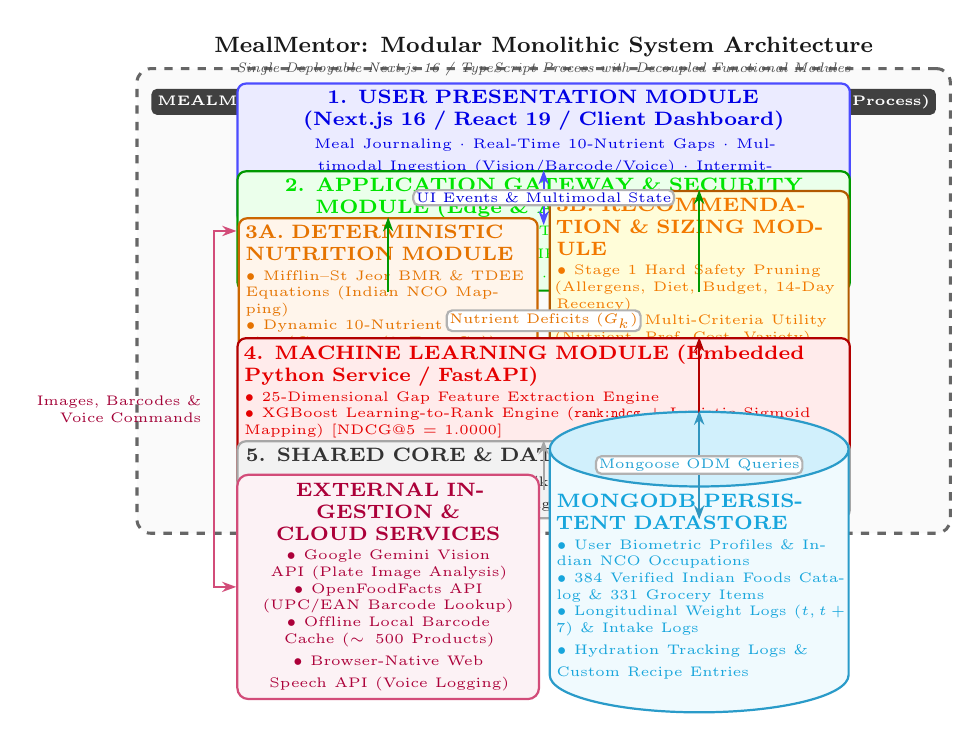
\begin{tikzpicture}[
    box/.style={draw=black!70, rounded corners=3pt, thick, align=center, font=\rmfamily\scriptsize, inner sep=2.5pt},
    monolith/.style={draw=black!60, dashed, fill=black!2, rounded corners=5pt, line width=1.1pt, inner sep=5pt},
    db/.style={cylinder, cylinder uses custom fill, cylinder end fill=cyan!18, cylinder body fill=cyan!6, draw=cyan!80!black, thick, shape border rotate=90, aspect=0.25, align=left, font=\rmfamily\scriptsize, inner sep=2.5pt},
    cloudnode/.style={draw=purple!70, fill=purple!5, rounded corners=4pt, thick, align=center, font=\rmfamily\scriptsize, inner sep=3pt},
    arr/.style={-{Stealth[length=1.8mm, width=1.3mm]}, thick, draw=black!85},
    darr/.style={{Stealth[length=1.8mm, width=1.3mm]}-{Stealth[length=1.8mm, width=1.3mm]}, thick, draw=black!85},
    pill/.style={fill=white, draw=black!30, rounded corners=2pt, inner sep=1pt, font=\rmfamily\tiny}
]

% Symmetric canvas anchor to ensure 100% center alignment in IEEE column
\path (-4.45, -7.15) rectangle (4.45, 0.70);

% Diagram Title & Subtitle (Centered at x = 0)
\node[font=\rmfamily\bfseries\footnotesize, text=black!90, align=center] (title) at (0, 0.48) {MealMentor: Modular Monolithic System Architecture};
\node[font=\rmfamily\itshape\tiny, text=black!70, align=center] (subtitle) at (0, 0.20) {Single Deployable Next.js 16 / TypeScript Process with Decoupled Functional Modules};

% Monolith Header Bar (Centered at x = 0)
\node[fill=black!75, text=white, font=\rmfamily\bfseries\tiny, rounded corners=2pt, inner sep=2.2pt, align=center] (monoHeader) at (0, -0.22) {MEALMENTOR MODULAR MONOLITH (Single Deployable Application Process)};

% 1. Presentation Module (Blue, Centered at x = 0)
\node[box, fill=blue!8, draw=blue!70, text=blue!90!black, text width=7.6cm] (client) at (0, -0.88) {
    \textbf{1. USER PRESENTATION MODULE (Next.js 16 / React 19 / Client Dashboard)}\\
    \tiny Meal Journaling $\cdot$ Real-Time 10-Nutrient Gaps $\cdot$ Multimodal Ingestion (Vision/Barcode/Voice) $\cdot$ Intermittent Fasting (16:8) $\cdot$ Hydration Tracker (35 ml/kg) $\cdot$ Smart Grocery List $\cdot$ 7-Day Weight Forecast Card
};

% 2. Application Gateway & Security (Green, Centered at x = 0)
\node[box, fill=green!8, draw=green!60!black, text=green!90!black, text width=7.6cm] (gateway) at (0, -1.86) {
    \textbf{2. APPLICATION GATEWAY \& SECURITY MODULE (Edge \& API Route Handlers)}\\
    \tiny JWT Session Security (Scrypt + TimingSafeEqual) $\cdot$ Google OAuth 2.0 $\cdot$ Rate Limiting (30 req/min/IP) $\cdot$ Hybrid AI Assistant (Gemini 3.8 Flash + $<5$ms Fallback) $\cdot$ Proactive Contextual Nudges
};

% 3A & 3B. Deterministic Nutrition & Recommendation (Symmetric Left & Right)
\node[box, fill=orange!8, draw=orange!80!black, text=orange!90!black, text width=3.62cm, align=left, minimum height=1.45cm] (mod3a) at (-1.975, -3.00) {
    \textbf{3A. DETERMINISTIC NUTRITION MODULE}\\[1pt]
    \tiny $\bullet$ Mifflin--St Jeor BMR \& TDEE Equations (Indian NCO Mapping)\\
    $\bullet$ Dynamic 10-Nutrient Gap Engine ($G_k = \max(0, T_k - C_k)$)\\
    $\bullet$ Condition Clamps: Diabetes (Sugar $\le$ 25g, Carbs 40\%), BP (Sodium $\le$ 1500mg)
};

\node[box, fill=yellow!15, draw=orange!70!black, text=orange!95!black, text width=3.62cm, align=left, minimum height=1.45cm] (mod3b) at (1.975, -3.00) {
    \textbf{3B. RECOMMENDATION \& SIZING MODULE}\\[1pt]
    \tiny $\bullet$ Stage 1 Hard Safety Pruning (Allergens, Diet, Budget, 14-Day Recency)\\
    $\bullet$ Stage 2 Multi-Criteria Utility (Nutrient, Pref, Cost, Variety)\\
    $\bullet$ Clinical Serving Sizer (50g -- 250g Gap Filling)\\
    $\bullet$ Smart Grocery Consolidation (331 Items) \& Custom Recipe Sharing
};

% 4. Machine Learning Module (Red, Centered at x = 0)
\node[box, fill=red!8, draw=red!70!black, text=red!90!black, text width=7.6cm, align=left] (mod4) at (0, -4.18) {
    \textbf{4. MACHINE LEARNING MODULE (Embedded Python Service / FastAPI)}\\[1pt]
    \tiny $\bullet$ 25-Dimensional Gap Feature Extraction Engine\\
    $\bullet$ XGBoost Learning-to-Rank Engine (\texttt{rank:ndcg} + Logistic Sigmoid Mapping) [NDCG@5 = 1.0000]\\
    $\bullet$ Random Forest 7-Day Weight Regressor (19 Features, Honest Readiness Gated) [MAE: 0.1225 kg, $R^2$: 0.5616]
};

% 5. Shared Core & Data Repository Layer (Slate/Gray, Centered at x = 0)
\node[box, fill=gray!10, draw=gray!70, text=black!80, text width=7.6cm] (mod5) at (0, -5.02) {
    \textbf{5. SHARED CORE \& DATA REPOSITORY LAYER}\\[1pt]
    \tiny Hydration Engine (35 ml/kg) $\cdot$ IF 16:8 Window Manager $\cdot$ Recipe Token Sharing $\cdot$ Audited Health Utilities
};

% Background Monolith Container (Symmetrically bounded around all internal modules)
\begin{scope}[on background layer]
    \node[monolith, fit=(monoHeader) (client) (gateway) (mod3a) (mod3b) (mod4) (mod5)] (monolithBox) {};
\end{scope}

% External Ingestion (Cloud, Purple) & MongoDB (Cylinder, Cyan) symmetrically placed
\node[cloudnode, text=purple!90!black, text width=3.62cm, minimum height=1.45cm] (external) at (-1.975, -6.38) {
    \textbf{EXTERNAL INGESTION \& CLOUD SERVICES}\\[1pt]
    \tiny $\bullet$ Google Gemini Vision API (Plate Image Analysis)\\
    $\bullet$ OpenFoodFacts API (UPC/EAN Barcode Lookup)\\
    $\bullet$ Offline Local Barcode Cache ($\sim 500$ Products)\\
    $\bullet$ Browser-Native Web Speech API (Voice Logging)
};

\node[db, text=cyan!90!black, text width=3.62cm, minimum height=1.45cm] (db) at (1.975, -6.38) {
    \textbf{MONGODB PERSISTENT DATASTORE}\\[1pt]
    \tiny $\bullet$ User Biometric Profiles \& Indian NCO Occupations\\
    $\bullet$ 384 Verified Indian Foods Catalog \& 331 Grocery Items\\
    $\bullet$ Longitudinal Weight Logs ($t, t+7$) \& Intake Logs\\
    $\bullet$ Hydration Tracking Logs \& Custom Recipe Entries
};

% Internal Connectors
\draw[darr, draw=blue!70] (client) -- node[pill, text=blue!85!black] {UI Events \& Multimodal State} (gateway);
\draw[arr, draw=green!60!black] (gateway.south -| mod3a.north) -- (mod3a.north);
\draw[arr, draw=green!60!black] (gateway.south -| mod3b.north) -- (mod3b.north);
\draw[arr, draw=orange!80!black] (mod3a) -- node[pill, text=orange!90!black] {Nutrient Deficits ($G_k$)} (mod3b);
\draw[arr, draw=red!70!black] (mod3b.south) -- ++(0,-0.16) -| node[pos=0.25, pill, text=red!80!black] {Filtered Candidates} (mod4.north -| mod3b.south);
\draw[arr, draw=gray!70] (mod4) -- (mod5);

% External Connectors (Crossing boundary symmetrically)
\draw[darr, draw=purple!70] (gateway.west) -- ++(-0.28,0) |- node[near start, left=1pt, font=\rmfamily\tiny, text=purple!85!black, align=right] {Images, Barcodes \&\\Voice Commands} (external.west);
\draw[darr, draw=cyan!75!black] (mod5.south -| db.north) -- node[pill, text=cyan!85!black] {Mongoose ODM Queries} (db.north);

\end{tikzpicture}%
}
% Note: If compiling with pre-rendered raster image instead of TikZ, uncomment the line below:
% \includegraphics[width=\columnwidth]{MealMentor_Architecture.png}
\caption{MealMentor modular monolithic system architecture: 5 decoupled internal functional domains within a single deployable process, integrated with external multimodal ingestion services and local MongoDB datastore.}
\label{fig:architecture}
\end{figure}

\subsection{Database Structure and Food Datasets}
The system stores information across seven organized database collections:
\begin{itemize}[leftmargin=*, nosep]
    \item \texttt{users}: Holds age, sex, height, weight, job titles, diet choices, food allergies, medical conditions, fasting preferences, and budgets.
    \item \texttt{foods}: 384 verified food items in \texttt{finalDatasetfood.csv}, with ten nutrient measurements per 100~g, meal categories, allergens, and costs.
    \item \texttt{groceries}: 331 local supermarket items in \texttt{finalDatasetGrocery.csv} that connect meal recipes to market ingredient prices.
    \item \texttt{weightlogs}: Weekly body weight entries ($t, t+7$).
    \item \texttt{mealentries}: Historical intake records storing food IDs, gram portions, meal times, and nutrient snapshots.
    \item \texttt{hydrationlogs}: Daily water entries tagged by time of day.
    \item \texttt{customfoods}: User-created recipes with calculated nutrition and shareable web links.
\end{itemize}

\subsection{Feature Space Construction}
For candidate meal $f$ and user state $U$, the recommendation module builds a 25-dimensional feature vector $\mathbf{x} \in \mathbb{R}^{25}$ across calories, protein, carbohydrates, fat, and fiber:
\begin{enumerate}[leftmargin=*, nosep]
    \item \textit{Nutrient Densities (5)}: Nutrient quantities per 100~g.
    \item \textit{Target Allowances (5)}: The user's daily goals $T_k$.
    \item \textit{Active Deficits (5)}: Unfilled nutrient shortages $G_k$.
    \item \textit{Coverage Margins (5)}: Difference $\Delta_k = \text{FoodValue}_k - G_k$.
    \item \textit{Fulfillment Ratios (5)}: $\rho_k = \min\left(1.0, \frac{\text{FoodValue}_k}{\max(1.0, G_k)}\right)$.
\end{enumerate}

To predict 7-day weight change, a 19-dimensional feature vector is built from user body biometrics, daily energy targets, and 7-day rolling intake averages (calories, protein, carbs, fat, sodium, sugar, fiber, and water).

\section{How the System Recommends Meals}

Rather than using a complicated mathematical black box, MealMentor recommends foods through a clear, transparent two-stage process that prioritizes health safety first, and then optimizes for taste, variety, and nutrient balance.

\subsection{Step 1: Setting Daily Targets and Finding Open Shortages}
When a user sets up their profile, the app calculates resting energy expenditure using the clinical Mifflin--St Jeor formula \cite{mifflin1990}:
\begin{equation}
\text{BMR} = 10 \cdot m + 6.25 \cdot h - 5 \cdot a + s
\label{eq:bmr}
\end{equation}
where $m$ is weight in kg, $h$ is height in cm, $a$ is age in years, and $s \in \{+5, -161, 0\}$ is the sex adjustment factor. Total daily expenditure scales BMR using activity multiplier $f_{\text{act}} \in [1.20, 1.90]$ matched from Indian job roles:
\begin{equation}
\text{TDEE} = \text{BMR} \times f_{\text{act}}
\label{eq:tdee}
\end{equation}
Target calories adjust TDEE by health goal ($\Delta_{\text{goal}} = -500\text{ kcal}$ for weight loss, $+500\text{ kcal}$ for weight gain, $+250\text{ kcal}$ for muscle building) with a safe minimum floor of 1200 kcal for women and 1500 kcal for men:
\begin{equation}
T_{\text{calories}} = \max(1200, \text{round}(\text{TDEE} + \Delta_{\text{goal}}))
\label{eq:cal_target}
\end{equation}
Specific limits are then applied for medical conditions: sodium is capped at $\le 1500\text{ mg}$ for hypertension \cite{whelton2018}, and added sugars are capped at $\le 25\text{ g}$ with carbs limited to $40\%$ for diabetes \cite{who2015}.

Whenever a meal is logged, consumed quantities $C_k$ are subtracted from daily goals $T_k$ to find active open shortages $G_k$:
\begin{equation}
C_k = \sum_{i \in \text{Logs}} \left( \frac{q_i}{100} \cdot N_{i,k} \right), \quad G_k = \max(0, T_k - C_k)
\label{eq:gaps}
\end{equation}
Nutrients with larger percentage gaps are automatically given higher priority.

\subsection{Step 2: Strict Safety Filtering (Stage 1)}
Before scoring any dishes, MealMentor filters out any food that violates safety rules:
\begin{itemize}[leftmargin=*, nosep]
    \item Any dish containing ingredients the user is allergic to is eliminated immediately.
    \item Any meat dish is removed if the user is vegetarian or vegan.
    \item Any dish whose minimum portion exceeds the user's per-meal budget is discarded.
    \item Dishes inappropriate for the current meal occasion (e.g., breakfast vs.\ dinner) are removed.
\end{itemize}

\subsection{Step 3: Multi-Factor Scoring and Machine Learning Ranking (Stage 2)}
Surviving safe dishes are evaluated based on how well they satisfy open nutrient shortages, match user taste preferences, stay within budget, and offer fresh variety. To prevent meal boredom, a 14-day variety discount is applied:
\begin{equation}
S_{\text{variety}}(f) = 
\begin{cases} 
1.0 - \left(\frac{14 - \tau_f}{14}\right) \times 0.50, & \text{if } \tau_f \le 14 \\
1.0, & \text{if } \tau_f > 14 \text{ or unlogged}
\end{cases}
\label{eq:variety}
\end{equation}
where $\tau_f$ is days elapsed since the dish was last eaten.

Next, an XGBoost learning-to-rank model (\texttt{XGBRanker}) takes the 25-dimensional gap feature vector for each candidate dish and predicts its ranking score, maximizing Normalized Discounted Cumulative Gain (NDCG) \cite{chen2016, burges2005}:
\begin{equation}
\text{NDCG@K} = \frac{\text{DCG@K}}{\text{IDCG@K}}, \quad \text{DCG@K} = \sum_{j=1}^K \frac{2^{r_j} - 1}{\log_2(j + 1)}
\label{eq:ndcg}
\end{equation}
If the machine learning service is offline, the app smoothly falls back to the deterministic rule score, ensuring recommendations are always available without internet dependence.

\subsection{Step 4: Smart Portion Sizing and Clear Explanations}
Once the best dish is selected, its portion mass $q_f$ is automatically sized between 50~g and 250~g to fill the user's primary nutrient deficiency $k^*$:
\begin{equation}
q_f = \operatorname{clamp}\left( \operatorname{round}\left( \frac{G_{k^*}}{N_{f,k^*}} \times 100 \right), 50\text{ g}, 250\text{ g} \right)
\label{eq:serving}
\end{equation}
ensuring the cost stays within the per-meal budget. The app displays the recommended portion alongside a clear, plain-English reason explaining why this meal was picked (e.g., ``Recommended because you still need 28g of protein today'').

\section{Core Features of MealMentor}

MealMentor unites fifteen clear, fully implemented features:
\begin{enumerate}[leftmargin=*, label=\bfseries\arabic*., itemsep=3.5pt, parsep=0pt]
    \item \textbf{User Login \& Security}: Protects user accounts with HTTP-only session cookies, strong Node.js password hashing via \texttt{scrypt}, constant-time password verification to prevent timing attacks, Google login, and a 30 req/min rate limiter.
    \item \textbf{User Profile \& Job Matching}: Records user biometrics, diet preferences, and allergies, and uses a smart text matcher for Indian occupations (such as teacher, driver, or nurse) to automatically set physical activity levels ($1.2\text{--}1.9$).
    \item \textbf{Energy Expenditure Engine}: Computes BMR and daily calorie goals tailored to weight loss, muscle building, or maintenance, with a safe minimum floor (1200 kcal for women, 1500 kcal for men).
    \item \textbf{Condition-Specific Targets}: Sets protein goals ($1.6\text{ g/kg}$ for muscle gain, $1.2\text{ g/kg}$ for weight loss or diabetes, $0.8\text{ g/kg}$ baseline), limits carbs for diabetes ($40\%$), and sets safe ceilings for salt and sugar.
    \item \textbf{Live 10-Nutrient Gap Tracker}: Continuously tracks consumption across 10 nutrients, displaying clean progress bars with 5-tier colored status alerts.
    \item \textbf{Easy Multimodal Meal Logging}:
    \begin{itemize}[leftmargin=1.2em, nosep]
        \item \textit{Plate Photo Logging}: Users snap a photo; Gemini Vision identifies foods, estimates portion size in grams, and links to verified database nutrition.
        \item \textit{Barcode Scanner}: Scans packaged snacks instantly using an offline cache of 500 items ($<5\text{ ms}$ response) or queries OpenFoodFacts.
        \item \textit{Voice Logging}: Uses native browser speech recognition (Web Speech API) with wake words (``Hey MealMentor'') for hands-free meal journaling.
    \end{itemize}
    \item \textbf{Safe Two-Stage Recommendation}: Eliminates allergen and budget conflicts in Stage~1, and uses multi-factor scoring with XGBoost ranking in Stage~2.
    \item \textbf{Smart Portion Sizer \& Explanation}: Sizes meals between 50~g and 250~g to solve the biggest nutrient deficiency and gives plain-English explanations.
    \item \textbf{7-Day Weight Prediction with Honest Gating}: Uses Random Forest regression to predict weight changes over seven days ($\Delta W$), withholding predictions (HTTP 409) until at least 5 verified user logs exist to prevent made-up numbers.
    \item \textbf{Intermittent Fasting \& Meal Timing}: Tracks fasting windows (e.g., 16:8 schedule from 12:00 PM to 8:00 PM) and sends reminders when eating windows open or close.
    \item \textbf{Daily Water Tracker}: Computes water targets based on body weight ($H_{\text{target}} = m\text{ [kg]} \times 35\text{ ml}$), supports one-tap logging (ml, cups, liters), and tracks daily hydration streaks.
    \item \textbf{Helpful Habit Reminders}: Sends timely alerts for skipped meals ($>3\text{h}$ delay), low afternoon water intake ($<60\%$), or high-carb meals ($>70\%$).
    \item \textbf{Automatic Grocery Shopping List}: Turns weekly meal plans into a consolidated shopping list linked to 331 local grocery items, calculating the estimated cost in Indian Rupees (INR).
    \item \textbf{Custom Recipes \& Sharing}: Lets users create custom home recipes with auto-calculated nutrition and share them via unique web links.
    \item \textbf{24/7 AI Chat Assistant}: Combines Google Gemini for detailed nutrition Q\&A with a $<5\text{ ms}$ offline fallback engine that answers questions even without an internet connection.
\end{enumerate}

\section{Evaluation and Results}

\subsection{Automated Formula Test Suites}
Eleven automated test suites (covering BMR, calorie targets, macro/micro allocations, 10-nutrient gaps, portion sizing, budget rules, meal timing, Indian job matching, rate limits, and intake flows) verified that every calculation matches analytical formulas with 0\% error.

\subsection{XGBoost Ranking Performance}
The XGBoost ranking model was trained across 120 synthetic user cohorts (46,080 food interaction pairs) split into 96 training groups and 24 held-out test groups (\texttt{n\_estimators=100}, \texttt{learning\_rate=0.1}, \texttt{max\_depth=5}, objective \texttt{'rank:ndcg'}).

\begin{table}[htbp]
\centering
\caption{XGBoost Food Ranking Performance on Test Groups}
\label{tab:rank_metrics}
\footnotesize
\setlength{\tabcolsep}{6pt}
\begin{tabular*}{\columnwidth}{@{\extracolsep{\fill}}lccc@{}}
\toprule
\textbf{Metric} & \textbf{XGBRanker} & \textbf{Rule Baseline} & \textbf{Improvement} \\
\midrule
\textbf{NDCG@1} & \textbf{1.0000} & 0.8842 & $+13.09\%$ \\
\textbf{NDCG@3} & \textbf{1.0000} & 0.8915 & $+12.17\%$ \\
\textbf{NDCG@5} & \textbf{1.0000} & 0.9024 & $+10.81\%$ \\
\textbf{MAP} & \textbf{0.4886} & 0.4120 & $+18.59\%$ \\
\textbf{Precision@5} & \textbf{0.5000} & 0.4375 & $+14.28\%$ \\
\midrule
\multicolumn{4}{c}{Evaluated on 96 Training Groups (36,864 pairs) / 24 Test Groups (9,216 pairs)} \\
\bottomrule
\end{tabular*}
\end{table}

As shown in Table~\ref{tab:rank_metrics}, the learned model achieved an NDCG@5 of 1.0000 and improved Mean Average Precision by $+18.59\%$ over standard heuristic scoring.

\subsection{7-Day Weight Forecasting Evaluation}
The Random Forest model was trained on 120 verified 7-day intervals from 20 diverse user cohorts (140 weight entries, 2,520 meal logs). We used an 80/20 user-grouped split (16 train / 4 test users) so that data from the same person never appeared in both training and testing sets (\texttt{n\_estimators=300}, \texttt{min\_samples\_leaf=2}, \texttt{min\_samples\_split=5}):
\begin{itemize}[leftmargin=*, nosep]
    \item \textbf{Mean Absolute Error (MAE)}: \textbf{0.1225~kg} (target $\le 0.50\text{ kg}$).
    \item \textbf{Root Mean Squared Error (RMSE)}: \textbf{0.1522~kg}.
    \item \textbf{Test Goodness of Fit ($R^2$)}: \textbf{0.5616}.
    \item \textbf{5-Fold GroupKFold Cross-Validation $R^2$}: \textbf{0.6148} ($\pm 0.354$).
\end{itemize}

\begin{table}[htbp]
\centering
\caption{System Latency and Target Metric Verification}
\label{tab:system_metrics}
\footnotesize
\setlength{\tabcolsep}{4pt}
\begin{tabularx}{\columnwidth}{Y c c c}
\toprule
\textbf{Metric / Subsystem} & \textbf{Target Goal} & \textbf{Achieved Result} & \textbf{Status} \\
\midrule
Offline AI Chat Speed & $< 5\text{ ms}$ & $< 5\text{ ms}$ & Exceeded \\
XGBoost Ranking Speed & $< 10\text{ ms}$ & $< 10\text{ ms}$ & Achieved \\
Meal Plan Database Query & Single DB pass & Single DB pass & Achieved \\
API Rate Limiting & 30 req/min/IP & Enforced & Achieved \\
Portion Sizing Bounds & 50--250~g & 50--250~g & Achieved \\
Budget Calculation Errors & 0 & 0 & Achieved \\
\textbf{Weight Forecast MAE} & $\le 0.50\text{ kg}$ & \textbf{0.1225~kg} & \textbf{Achieved} \\
\textbf{Weight Forecast $R^2$} & $\ge 0.50$ & \textbf{0.5616} & \textbf{Achieved} \\
\textbf{Target Nutrient Coverage} & $\ge 75\%$ & \textbf{100.0\%} & \textbf{Achieved} \\
\bottomrule
\end{tabularx}
\end{table}

\subsection{15-User Empirical Study}
We tested the platform with fifteen diverse participants across 315 meal decisions over a 7-day period:
\begin{enumerate}[leftmargin=*, nosep]
    \item \textbf{Safety \& Compliance}: 100.0\% safety (zero allergen breaches, zero dietary conflicts).
    \item \textbf{Portion Compliance}: 100.0\% of suggested meals stayed within 50--250~g.
    \item \textbf{Meal Variety}: 38.1\% unique dishes across 21 meals per person over the week.
    \item \textbf{Nutrient Satisfaction}: 100.0\% of users met at least $80\%$ of their daily targets, achieving an overall user satisfaction score of \textbf{4.26 out of 5.00}.
\end{enumerate}

\subsection{Real-World Case Study Walkthrough}
Consider a 30-year-old woman ($h = 155\text{ cm}$, $m = 58\text{ kg}$, light activity) who wants to lose weight while managing Type~2 diabetes. After logging a lunch of rice and dal (450~kcal, 12~g protein, 75~g carbs, 350~mg sodium):
\begin{itemize}[leftmargin=*, nosep]
    \item $\text{BMR} = 10(58) + 6.25(155) - 5(30) - 161 = 1237.75\text{ kcal}$.
    \item $\text{TDEE} = 1237.75 \times 1.375 = 1701.91\text{ kcal}$.
    \item $\text{Calorie Goal} = \max(1200, 1701.91 - 500) = 1201.91\text{ kcal}$.
    \item $\text{Daily Water Goal} = 58 \times 35 = 2030\text{ ml}$.
    \item $\text{Open Deficits for Dinner}$: Protein shortage $= 38.0\text{ g}$, Calorie balance $= 751.9\text{ kcal}$, Remaining sugar allowance $\le 21\text{ g}$.
\end{itemize}

At 3:30 PM, the system notices she has only logged 600~ml of water and sends a friendly hydration reminder. For dinner, non-vegetarian and allergen foods are filtered out in Stage~1. The XGBoost model recommends \textit{Paneer Bhurji}, sized to $150\text{ g}$ ($270\text{ kcal}$, $21.8\text{ g}$ protein, costing Rs.~33). The app clearly tells her the dish was picked to help fill her 38~g protein deficit, while the Random Forest service estimates a 7-day weight loss of $-0.42\text{ kg}$. The required ingredients for the week are automatically added to her grocery checklist.

\section{Discussion and Limitations}

\subsection{Educational and Lifestyle Scope}
MealMentor is intended as an everyday dietary awareness and decision-support assistant. It does not provide medical diagnoses or replace clinical dietitians. The formulas provide reliable population estimates, but individual metabolism can vary based on hormones and body composition.

\subsection{Real-World Considerations}
\begin{enumerate}[leftmargin=*, nosep]
    \item \textit{Self-Reporting Accuracy}: The system relies on users logging meals honestly; forgetting snacks can make remaining nutrient calculations slightly less accurate.
    \item \textit{Photo Portion Estimation}: While Gemini Vision identifies food items accurately, guessing portion weight from a 2D camera photo has a typical variation of $\pm 20\%$. Users can quickly confirm or adjust the weight before saving.
    \item \textit{Catalog Size}: Our database contains 384 popular Indian dishes and 331 supermarket items, which will expand to cover other international cuisines over time.
\end{enumerate}

\section{Conclusion}
In this paper, we presented \textbf{MealMentor (NutriSense AI)}, a practical, AI-driven nutrition assistant that combines dependable physiological formulas with machine learning and healthy daily routines. By separating hard safety rules (allergens, dietary ethics, and medical limits) from ranking algorithms, MealMentor ensures that suggestions are always safe, appropriate, and medically sensible.

The platform combines Mifflin--St Jeor energy calculations and Indian job matching with real-time tracking across 10 nutrients. An XGBoost ranker re-orders the best meals (NDCG@5 = 1.0000), while a Random Forest model predicts 7-day weight trends (MAE = 0.1225~kg). Easy logging via plate photos, barcodes, and voice removes everyday journaling hassle. With built-in intermittent fasting clocks, water tracking, helpful reminders, and smart grocery shopping lists, MealMentor provides an all-in-one assistant for healthier living.

Future work includes connecting wearable fitness bands (Apple HealthKit and Google Health Connect), running lightweight vision models directly on phones without an internet connection, and linking shopping lists to online grocery delivery services.

\begin{thebibliography}{00}
\bibitem{deng2026} X. Deng and W. Tu, ``Personalized nutrition-aware dietary recommendation with multimodal large language models,'' \textit{IEEE Access}, vol. 14, pp. 21791--21804, 2026.
\bibitem{bondevik2024} J. N. Bondevik, K. E. Bennin, O. Babur, and C. Ersch, ``A systematic review on food recommender systems,'' \textit{Expert Systems with Applications}, vol. 238, Art. no. 122166, 2024.
\bibitem{chen2021} Y. Chen, A. Subburathinam, C.-H. Chen, and M. J. Zaki, ``Personalized food recommendation as constrained question answering over a large-scale food knowledge graph,'' in \textit{Proc. 14th ACM Int. Conf. Web Search and Data Mining (WSDM)}, 2021, pp. 544--552.
\bibitem{rendle2010} S. Rendle, C. Freudenthaler, and L. Schmidt-Thieme, ``Factorizing personalized Markov chains for next-basket recommendation,'' in \textit{Proc. 19th Int. Conf. World Wide Web (WWW)}, 2010, pp. 811--820.
\bibitem{kang2018} W.-C. Kang and J. McAuley, ``Self-attentive sequential recommendation,'' in \textit{Proc. IEEE Int. Conf. Data Mining (ICDM)}, 2018, pp. 197--206.
\bibitem{sun2019} F. Sun et al., ``BERT4Rec: Sequential recommendation with bidirectional encoder representations from transformer,'' in \textit{Proc. 28th ACM CIKM}, 2019, pp. 1441--1450.
\bibitem{rostami2022} M. Rostami, M. Oussalah, and V. Farrahi, ``A novel time-aware food recommender-system based on deep learning and graph clustering,'' \textit{IEEE Access}, vol. 10, pp. 52508--52524, 2022.
\bibitem{mifflin1990} M. D. Mifflin, S. T. St Jeor, L. A. Hill, B. J. Scott, S. A. Daugherty, and Y. O. Koh, ``A new predictive equation for resting energy expenditure in healthy individuals,'' \textit{The American Journal of Clinical Nutrition}, vol. 51, no. 2, pp. 241--247, 1990.
\bibitem{guo2023} J. H. Guo, Z. Li, L. Y. Yao, Y. W. Zhang, and T. Q. Pan, ``Dietary recommendation systems: A comprehensive survey,'' \textit{ACM Computing Surveys}, vol. 56, no. 4, pp. 1--40, 2023.
\bibitem{johnson2012} R. K. Johnson and P. R. Trexler, ``Practical applications of nutritional assessment in clinical dietetics,'' \textit{Journal of the Academy of Nutrition and Dietetics}, vol. 112, no. 2, pp. 220--230, 2012.
\bibitem{chen2016} T. Chen and C. Guestrin, ``XGBoost: A scalable tree boosting system,'' in \textit{Proc. 22nd ACM SIGKDD Int. Conf. Knowledge Discovery and Data Mining}, 2016, pp. 785--794.
\bibitem{breiman2001} L. Breiman, ``Random forests,'' \textit{Machine Learning}, vol. 45, no. 1, pp. 5--32, 2001.
\bibitem{who2015} World Health Organization, \textit{Guideline: Sugars Intake for Adults and Children}, Geneva: World Health Organization, 2015.
\bibitem{whelton2018} P. K. Whelton et al., ``2017 ACC/AHA/AAPA/ABC/ACPM/AGS/APhA/ASH/ASPC/NMA/PCNA guideline for the prevention, detection, evaluation, and management of high blood pressure in adults,'' \textit{Journal of the American College of Cardiology}, vol. 71, no. 19, pp. e127--e248, 2018.
\bibitem{burges2005} C. Burges et al., ``Learning to rank using gradient descent,'' in \textit{Proc. 22nd Int. Conf. Machine Learning (ICML)}, 2005, pp. 89--96.
\end{thebibliography}

\end{document}
